%% %%%%%%%%%%%%%%%%%%%%%%%%%%%%%%%%%%%%%%%%%%%%%%%%
%% Problem Set/Assignment Template to be used by the
%% Food and Resource Economics Department - IFAS
%% University of Florida's graduates.
%% %%%%%%%%%%%%%%%%%%%%%%%%%%%%%%%%%%%%%%%%%%%%%%%%
%% Version 1.0 - November 2019
%% %%%%%%%%%%%%%%%%%%%%%%%%%%%%%%%%%%%%%%%%%%%%%%%%
%% Ariel Soto-Caro
%%  - asotocaro@ufl.edu
%%  - arielsotocaro@gmail.com
%% %%%%%%%%%%%%%%%%%%%%%%%%%%%%%%%%%%%%%%%%%%%%%%%%

\documentclass[12pt]{article}
\usepackage{design_ASC}

\setlength\parindent{0pt} %% Do not touch this

%% -----------------------------
%% TITLE
%% -----------------------------
\title{IDbyDNA code challange} %% Title

\author{Hanie Samimi}%% Author's name

\date{\today} %% Change "\today" by another date manually
%% -----------------------------
%% -----------------------------

%% %%%%%%%%%%%%%%%%%%%%%%%%%
\begin{document}
\setlength{\droptitle}{-5em}    
%% %%%%%%%%%%%%%%%%%%%%%%%%%
\maketitle

% --------------------------
% Start here
% --------------------------

% %%%%%%%%%%%%%%%%%%%
\section*{Question 3}
% %%%%%%%%%%%%%%%%%%%
{\bfseries In your own words, write a brief technical methods section describing Sensitivity and Specificity as related to scoring the performance of a diagnostic test}

(LaTex is preferred)
% %%%%%%%%%%%%%%%%%%%
\subsection*{Answer}
% %%%%%%%%%%%%%%%%%%%
Diagnostic tests have different meanings in different fields. In general, a diagnostic test is
a tool to answer to a yes or no question about a sample condition. The answer should be determined based on sample features. For example, Body Mass Index (BMI) is a tool which determines if a person is overweight or not \cite{BMI}. The BMI uses height and current weight of each person and computes a relative score and classify people into different categories .
There could be a possibility that the answer is wrong but hypothesis is based on same features gathered from diagnostic tests. For instance, laboratory test such as surgery, can determine the presence of any symptoms in liver with highest accuracy. However, these tests have side effects too \cite{biopsy}.\\
An alternative solution could be using X-ray scan of the liver. To find the accuracy of the results of X-ray, we can use a confusion matrix. A confusion matrix is table that visualizes the classification of samples based on their actual and predicted condition using a diagnosis test\cite{CFT}. Below is a sample of confusion matrix for a group of 344 patients. Each row shows the classification based on X-ray scan while columns is based on laboratory tests \cite{table}.   

\begin{figure}
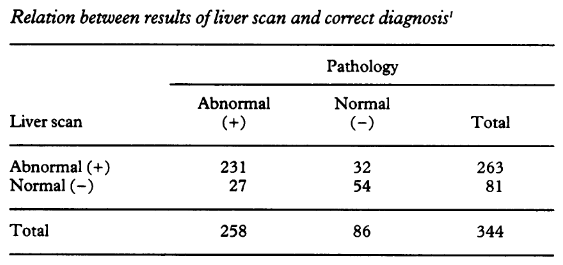
\includegraphics[width=\textwidth]{confusionMatrix.png}
\caption{Confusion matrix for liver cancer test. Rows show the classification based on X-ray test while columns are results based on laboratory test.} \label{fig1}
\end{figure}

The table shows that there are 231 cases that are predicted with liver abnormal condition based on both X-ray and laboratory test. However, there are 27 cases that have abnormality based on the laboratory test while X-ray test failed to identify them. On the other hand, there are 54 cases that have normal liver condition based on both X-ray and laboratory test. In addition, 32 cases were symptom free while X-ray test labeled them as Abnormal. 
These numbers show us the number of times that the X-ray was accurate as liver scan test. In order to score the accuracy of X-ray test and compare it alternative ones, we need to compute four values using the confusion matrix: 
\begin{center}
\begin{itemize}
\item True positive (TP): Number of Abnormal cases based on both tests 
\item True negative (TN): Number of Normal cases based on both test test
\item False positive (FP): Number of Normal cases that are predicted as Abnormal by x-ray test 
\item False negative (FN): Number of Abnormal cases that are predicted as normal by x-ray test
\end{itemize}
\end{center}
Figure 2 shows these four numbers for 231 cases of the study. 

\begin{figure}
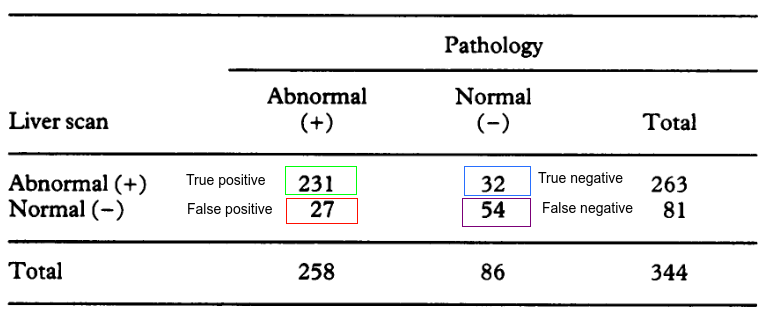
\includegraphics[width=\textwidth]{labeledCFT.png}
\caption{The confusion matrix is labeled with true positive, false negative, true negative and false positive labels} \label{fig1}
\end{figure}


These numbers are being used to compute two scores called Sensitivity and Specificity. These scores were first defined by Jacob Yerushalmy, an American bio-statistician in 1947 \cite{biostat}. Sensitivity or true-positive rate shows the ratio of abnormal cases that are diagnosed with symptom among to all cases that have been diagnosed with symptom. Specificity or true-negative rate is the ratio of normal cases that are diagnosed symptom free to all normal cases.\\
\begin{center}
$Sensitivity = TP / (TP+FN)$ \space $Specificity = TN / (TN + FP)$
\end{center}

In reality, there is a trade-off between increasing these two scores.Higher values of sensitivity shows that results for cases that are diagnosed with symptoms are reliable. Higher specificity shows that the chance of mislabeling normal case with an abnormal label is very low. To increase sensitivity, the tool will label cases with weak symptoms as abnormal. It will increase the chance of finding more abnormal case while increase the chance of mislabeling and decrease specificity. On the other hand, labeling normal to cases with weak symptoms decreases the chance of finding abnormal cases and results in lower sensitivity.
While these scores are important to select a test, they can not guarantee that tests results will be highly reliable for all situations. 

In conclusion, sensitivity and specificity score of a tool can determine the reliability of outcomes. However, interpreting these scores are dependent to the population of the study. While tools with higher sensitivity score  performs exceptionally well in specific number  population, but they will not work the same in other population.


\begin{thebibliography}{1}
\bibitem{biopsy}
Bravo, Arturo A., Sunil G. Sheth, and Sanjiv Chopra. "Liver biopsy." New England Journal of Medicine 344.7 (2001): 495-500.

\bibitem{table}
Drum, D. E. "Christacopoulos) S." Hepatic scintigraphy in clinical decision making. J Nucl Med1972 13: 908-15.

\bibitem{CFT}
Powers, David Martin. "Evaluation: from precision, recall and F-measure to ROC, informedness, markedness and correlation." (2011).

\bibitem{BMI}
Prentice, Andrew M., and Susan A. Jebb. "Beyond body mass index." Obesity reviews 2.3 (2001): 141-147.

\bibitem{biostat}
Yerushalmy, Jacob. "Statistical problems in assessing methods of medical diagnosis, with special reference to X-ray techniques." Public Health Reports (1896-1970) (1947): 1432-1449.




\end{thebibliography}
\smallskip

\end{document}